\section[Testy Wydajnościowe OpenCL na Urządzeniach z systemem Android]{Testy Wydajnościowe OpenCL na Urządzeniach z systemem Android}

\subsection[Pomiar Mocy Obliczeniowej]{Pomiar Mocy Obliczeniowej}
Pomiary mocy obliczeniowej zostaną przeprowadzone za pomocą następującego testu.
Wykonany zostanie jeden z poniższych kerneli. Wykorzystane zostaną wektorowe typy danych. Dla każdego z tych kerneli liczba wykonanych operacji zmiennoprzecinkowych powinna być taka sama i wynosić 4096 dla pojedynczego work itemu. W przykładowo kernelu flops\_float1 operacja mad zostanie wykonana 2048 razy funkcja ta składa się z pojedynczego mnożenia i dodawania.

\lstinputlisting{listings/flops_kernels.cl}

Argument kernela \_A to przykładowa, zmiennoprzecinkowa wartość początkowa. W przeprowadzonych testach rozmiar lokalnej work grupy to maksymalny możliwy rozmiar dla kernela. Natomiast rozmiar globalnej work grupy to największy możliwy rozmiar lokalnej grupy przemnożony przez liczbę dostępnych jednostek wykonawczych razy 2048.

Uzyskany wynik przedstawiony zostaje w jednostce FLOPS jest to jednostka określająca liczbę wykonanych operacji zmiennoprzecinkowych na sekundę. W tym teście wartość w FLOPS otrzymamy przez pomnożenie liczby globalnych work itemów przez liczbę wykonywanych zmiennoprzecinkowych operacji w każdym z nich, a następnie podzielenie uzyskanej wartości przez czas w jakim te się wykonywały. Do zmierzenia czasu wykorzystano obiekt tyu cl\_event. Po wykonaniu kernela zostały odczytane wartości CL\_PROFILING\_COMMAND\_START i CL\_PROFILING\_COMMAND\_END. Różnica tych wartości to czas wykonywania funkcji na urządzeniu.

Analogiczne kernele zostaną wykorzystane do przetestowania innych typów danych takich jak inteager half i double, jeśli te są wspierane przez testowane urządzenie.

\subsection[Przepływ pamięci]{Przepływ pamięci}
Zbadane zostało jak szybko dane zostają kopiowane pomiędzy różnymi obszarami pamięci. Do przetestowania został użyty prosty kernel.

\lstinputlisting{listings/copy_kernel.cl}
 
W wykonywanym kernelu dla pojedynczego work itemu kopiowana jest jedna komórka pamięci z bufora src do dst. Typ pojedynczego elementu bufora jest definiowany na etapie kompilacji. W tym przykładzie może być to jedna z wektorowych wersji typu float.

W teście stworzone zostają dwa bufory pierwszy posiada inicjalne dane a drugi jest pusty. Po wykonaniu kernela W drugim buforze znajdują się dane z pierwszego. Zebrane informacje o czasie z obiektu typu cl\_event pozwalają nam obliczyć z jaką prędkością w bajtach na sekundę dochodzi o transferu pamięci.
Analogicznie kernele używające buforów pamięci o typie danych integer half czy double zostaną także rzetestowane.

\subsection[Czas Oczekiwania na wykonanie kernela]{Czas Oczekiwania na wykonanie kernela}
W celu sprawdzenia czasu oczekiwania na rozpoczęcie wykonywania kernela, wykonany został następujący test. Wykonany jest dowolny kernel w testowanym scenariuszu następujący.

\lstinputlisting{listings/increment.cl}

Po wykonaniu kernela odczytane zostały wartości CL\_PROFILING\_COMMAND\_QUEUED i CL\_PROFILING\_COMMAND\_START. Różnica tych dwóch to czas potrzebny przesłanie kernela do urządzenia i rozpoczęcie jego wykonania. Kernel taki zostaje wykonany określoną ilość razy a wynik końcowy zostaje uśredniony.
\subsection[Transfer pamięci wbudowanymi funkcjami]{Transfer pamięci wbudowanymi funkcjami}
Do przetransferowania danych do bufora i z bufora pamięci w OpenCL możemy następujące funkcje:
 \begin{itemize}
	\item \textbf{clEnqueueReadBuffer} Po wykonaniu tej funkcji dane z pod wskazanej pamięci zostaną zapisane w podanym buforze, który potem może być wykorzystany w wykonywanym kernelu.
	\item \textbf{clEnqueueReadBuffer} Kopiuje dane w drugą stronę. Z bufora do wskazanego obszaru pamięci, dzięki temu możemy odczytać dane po wykonaniu kerneli na urządzeniu.
	\item \textbf{clEnqueueMapBuffer} Funkcja zwraca wskaźnik na pamięć pod którą została zmapowana pamięć z bufora
	\item \textbf{clEnqueueUnmapMemObject} Funkcja ta zmapuje pamięć spod wskaźnika zwróconego z clEnqueueMapBuffer lub clEnqueueMapImage do wskazanego bufora lub obrazka.
\end{itemize}
Wyżej wskazane funkcje wykonane zostaną określoną ilość razy, a z obiektu event zostaną zebrane dane dotyczące czasu wykonania. Uśredniony wynik z wykonania funkcji pokaże w jakim czasie urządzenie jest wstanie transferować dane pomiędzy kodem pamięcią po stronie aplikacji a pamięcią po stronie urządzenia.
\subsection[Mnożenie macierzy]{Mnożenie Macierzy}
Iloczyn macierzy to działanie matematyczne, które można w łatwy sposób podzielić na części, które mogą wykonywać się równolegle. Wyliczenie każdego elementu macierzy wynikowej może odbywać się niezależnie od innych. Zaimplementowano test, który wylicza każdy element w wynikowej macierzy jako osobny work item. Iloczyn macierzy przy użyciu OpenCL może być wykonany za pomocą następującego kernela
\lstinputlisting{listings/MatrixMul}
W zbudowanym teście wykonywany jest iloczyn dwóch macierzy o rozmiarach 1024x1024. Zmierzony zostaje czas w jakim udało się je przez siebie przemnożyć. Operacja wykonana jest określoną liczbę razy a wartość końcowa jest średnią z tych wykonań. Eksperyment powtórzony jest dla kilku rozmiarów lokalnych work grup. W zależności od właściwości urządzenia pierwsze wykonanie będzie miało maksymalną możliwą wartość lokalnej work grupy w wymiarze X. W kolejnym wykonaniu wartość w wymiarze X zmniejszona będzie dwukrotnie zmniejszona, natomiast w wymiarze Y będzie ona dwukrotnie zwiększona. W kolejnych iteracjach procedura wygląda tak samo, aż rozmiar work grupy w wymiarze X osiągnie wartość 1. Test ten ilustruje, jak dobór rozmiaru work grupy może mieć wpływ na czas wykonania kernela.
\subsection[OpenCL do filtrowania obrazu z cameraApi]{OpenCL do filtrowania obrazu z cameraApi}
Do wyświetlania obrazu z kamery na ekranie urządzenia z androidem, wykorzystała zostaną prosta aplikacja, która przekazuje teksture z openGL do obiektu kamery jako previewTexture tekstura tworzona w następujący sposób.
\lstinputlisting{listings/createTextureExternal.txt}
 Tekstura przekazana do kamery jest aktualizowana co każdą klatkę. Odświeżenie obiektu obrazka powoduje wywołanie metody która wyrenderuje uzyskany obrazek i go wyświetli. Odpowiedzialny za to jest ten fragment kodu.
 
\lstinputlisting{listings/drawImage.txt}
Kod ten wywoła vertex shader a następnie fragment shader, dzięki temu wyświetlone zostaną dwa trójkąty wypełnione zawartością obrazka.
\lstinputlisting{listings/shaders.txt}
Powyższy kod sprawia, że obraz z kamery jest wyświetlany na ekranie urządzenia. Jest to bazowa aplikacja, dzięki której możemy zweryfikować jak bardzo wykonywane kernele OpenCL używające pokazywanego obrazka wpłyną na ilość wyświetlanych klatek na sekundę.
\subsubsection[Konwersja obrazu z kamery do RGB w aplikacji]{Konwersja obrazu z kamery do RGB w aplikacji}
Standard OpenCL umożliwia prace na obrazkach w kernelach, jednakże te muszą być w formacie RGBA lub podobnych zawierające kanał czerwony zielony i niebieski. Niestety obraz z kamery zazwyczaj dostępny jest tylko w mediowym formacie YUV. Dlatego by móc wykorzystać obraz z kamery w kernelu OpenCL musimy przechwycić dane w formacie YUV a następnie przepisać je na format RGBA. W tym celu modyfikujemy kod bazowej aplikacji by ta tworzyła texturę typu GL\_TEXTURE\_2D zamiast GL\_TEXTURE\_EXTERNAL\_OES. Dane o obrazie zarejestrowanym z kamery przechwytujemy funkcją onPreviewFrame, która zostaje ustawiona jako previewCallback w obiekcie kamery. W tablicy byte[] data, przekazanej jako pierwszy argument znajduje się obrazek w formacie YUV. Konwersja z formatu YUV do RGBA wygląda następująco.
\lstinputlisting{listings/yuvToRgba}. Po wykonaniu tej funkcji w tablicy rgb[] znajduje sie obraz w formacie RGBA. W celu zaktualizowania danych w naszej wyświetlanej teksturze wołamy następującą metodę. 
\lstinputlisting{listings/UpdateTexture}
Po jej wykonaniu dane z tablicy texture\_data, w którym znajduje się obrazek w formacie RGBA, zostaną umieszczone w wyświetlanej teksturze.
Wykonywanie konwersji do RGBA po stronie aplikacji jest dużym obciążeniem wydajnościowym. By poprawić wydajność, konwersja została wykonywana przez kernel w OpenCL. Po stronie OpenCL stworzone zostają dwa bufory, do pierwszego kopiujemy dane z kamery, po wykonaniu dane z drugiego bufora kopiowane są tablicy, która później zostanie wpisana do tekstury.

Następnym usprawnieniem jest pisanie do wyświetlanej tekstury bezpośrenio z wykonywanego kernela. Dzięki temu oszczędzamy czas potrzebny na kopiowanie danych po wykonaniu kernela a następnie kopiowania ich do tekstury. Wystarczy, że kontekst OpenCL zostanie stworzony w oparciu o uchwyty na kontekstu OpenGLa, a do kernela zostanie przekazany współdzielony obraz. Różnicą wykonywanego kernela od wyżej prezentowanego kodu po stronie aplikacji są deklaracja kernela, która wygląda następująco.
\lstinputlisting{listings/OclConversionDeclaration}
By wyliczone wartości pixela zapisać w obiekcie obrazka należy sprowadzić je do postaci zdenoramlizowanej tj. do wartości z przedziału 0-1, a następnie wpisać je do obrazka funkcją write\_imagef.
\lstinputlisting{listings/WriteImageF}
Oto podgląd kamery po konwersji do RGB
\begin{figure}[H]
	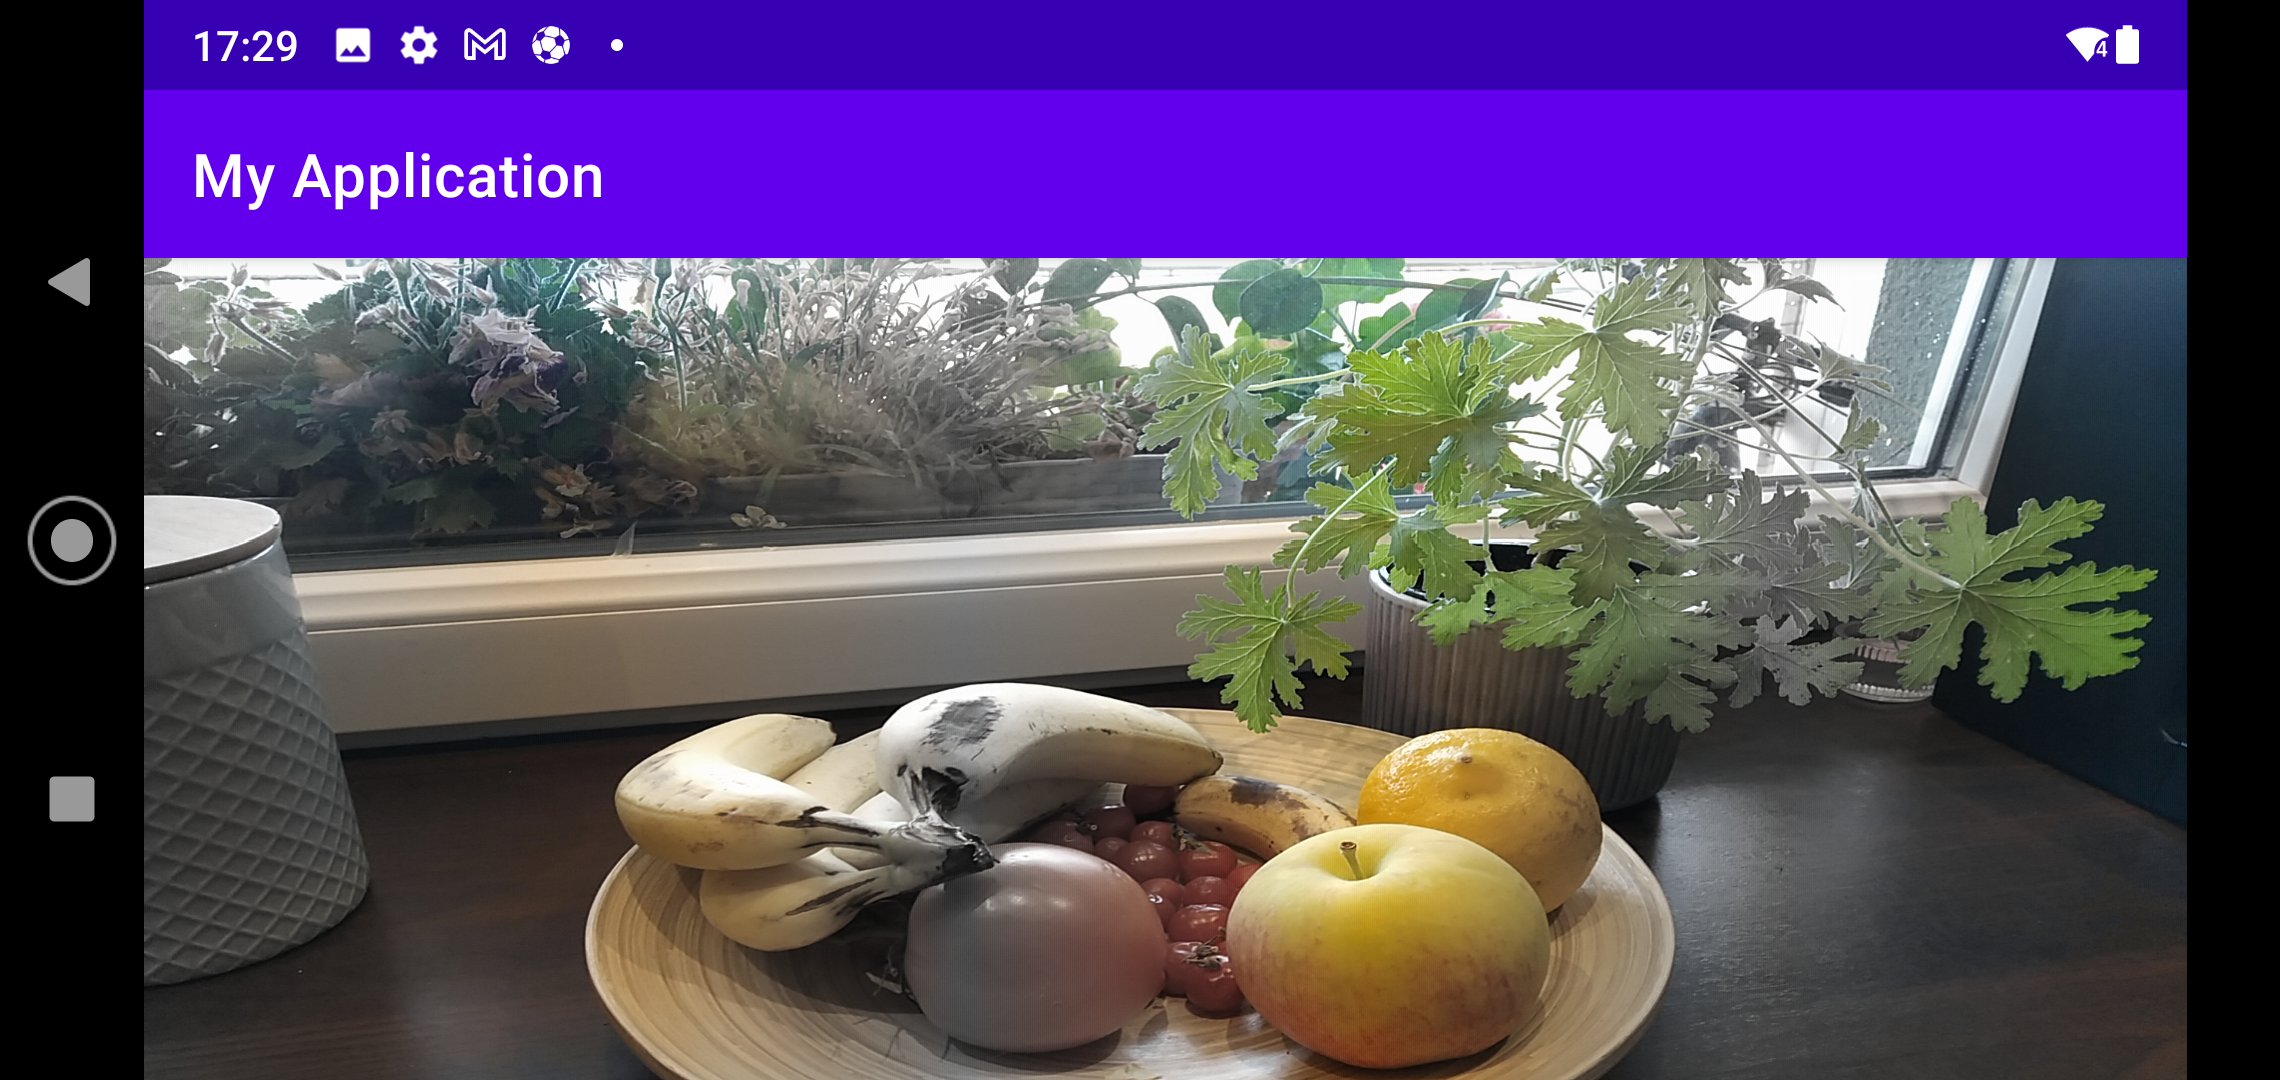
\includegraphics[scale=0.16]{imgs/preview.png}
	\caption{Podgląd Kamery}
\end{figure}
\subsubsection[Filtr Max Rgb]{Filtr Max Rgb}
Filtr Max RGB pozwala zwizualizować, który kanał posiada największą wartość dla danego piksela. By wykorzystać go przy wyświetlaniu obrazu z kamery należy uruchomić następujący kernel
\lstinputlisting{listings/maxRgb}
Filtr ten wybiera kanał z największą wartością i zeruje wartości w pozostałych. OpenCL nie pozwala na używanie tego samego obrazka do czytania i pisania. Dlatego do kernela przekazane zostają dwa obrazki. Pierwszy z możliwością zapisu, jest to obrazek wynikowy, później wyświetlony. Drugi to obrazek z możliwością odczytu posiadający dane obrazu z kamery urządzenia. Podgląd kamery po zastosowaniu filtru wygląda następująco.
\begin{figure}[H]
	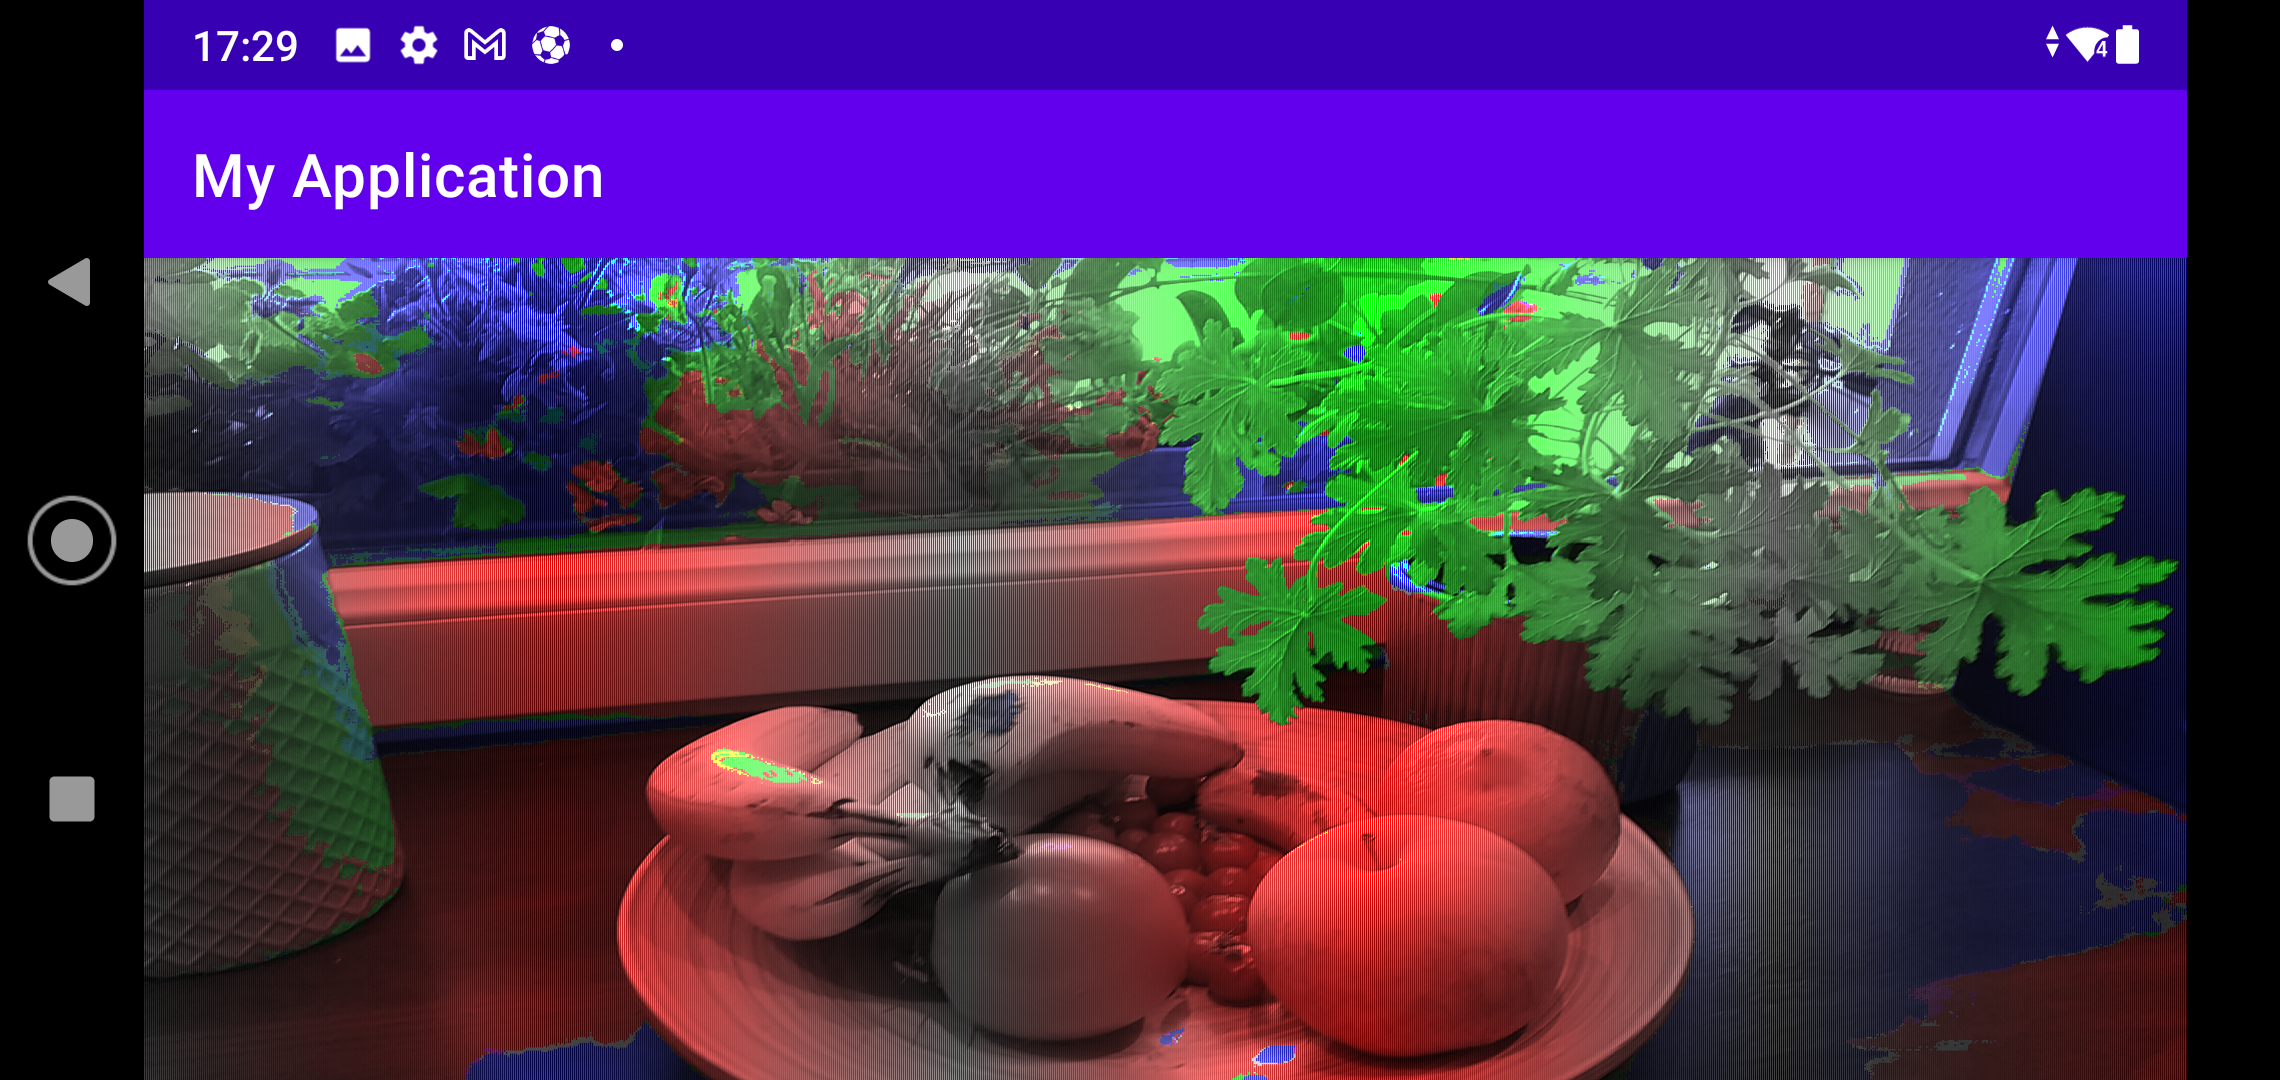
\includegraphics[scale=0.16]{imgs/maxRgb.png}
	\caption{Filtr Max Rgb}
\end{figure}
\subsubsection[Podgląd w skali szarości]{Podgląd w skali szarości}
Filtr pozwalający przedstawić obraz w skali szarości. By użyć filtra należy wykonać następujący kernel
\lstinputlisting{listings/grayScale.txt}
Kernel ten wylicza średnią wartość wszystkich kanałów, następnie tę wartość przypisuje każdemu z nich. Podgląd z kamery z tym filtrem wygląda następująco
\begin{figure}[H]
	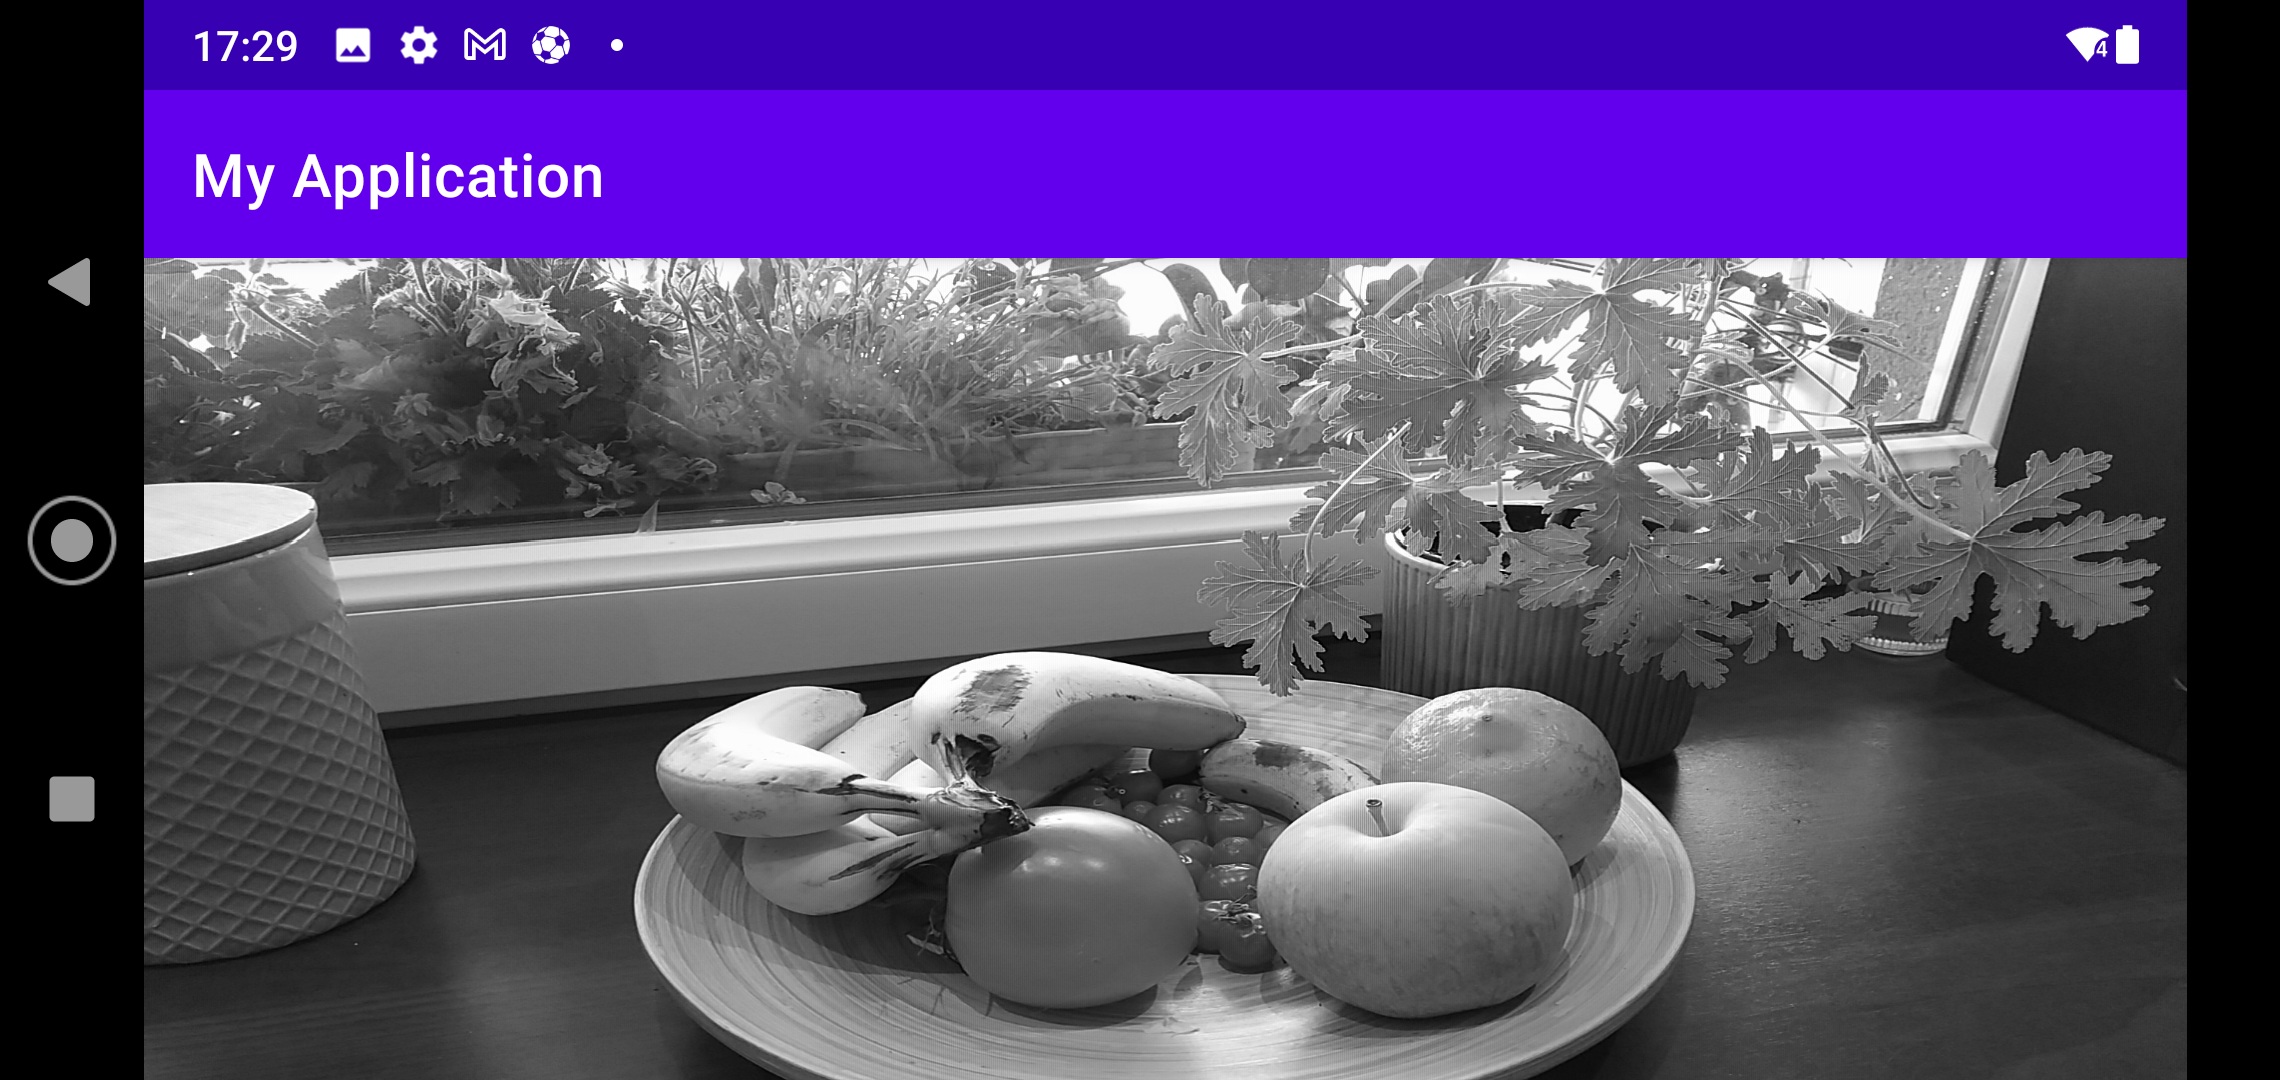
\includegraphics[scale=0.16]{imgs/BlackWhite.png}
	\caption{Podgląd w skali szarości}
\end{figure}
\subsubsection[Filtr Uśredniający]{Filtr Uśredniający}
Filtr Uśredniający polega na wyliczeniu wartości piksela na podstawie uśrednionej wartości pikseli sąsiadujących. Dzięki temu filtrowi dochodzi zmniejszenia różnic między sąsiednimi pikselami, przez co dochodzi do rozmycia obrazu i zmniejszenia kontrastu. Kernel nakładający filtr uśredniający wygląda następująco.
\lstinputlisting{listings/avgFilter}
Kernel ten wylicza średnią wartość pixeli w kwadracie 5x5 i wpisuje tą wartość do obrazu wynikowego. Dla każdego pixela zdjęcia źródłowego zostaje wyliczona jedna uśredniona wartość. Podgląd kamery z tym filtrem wygląda tak.
\begin{figure}[H]
	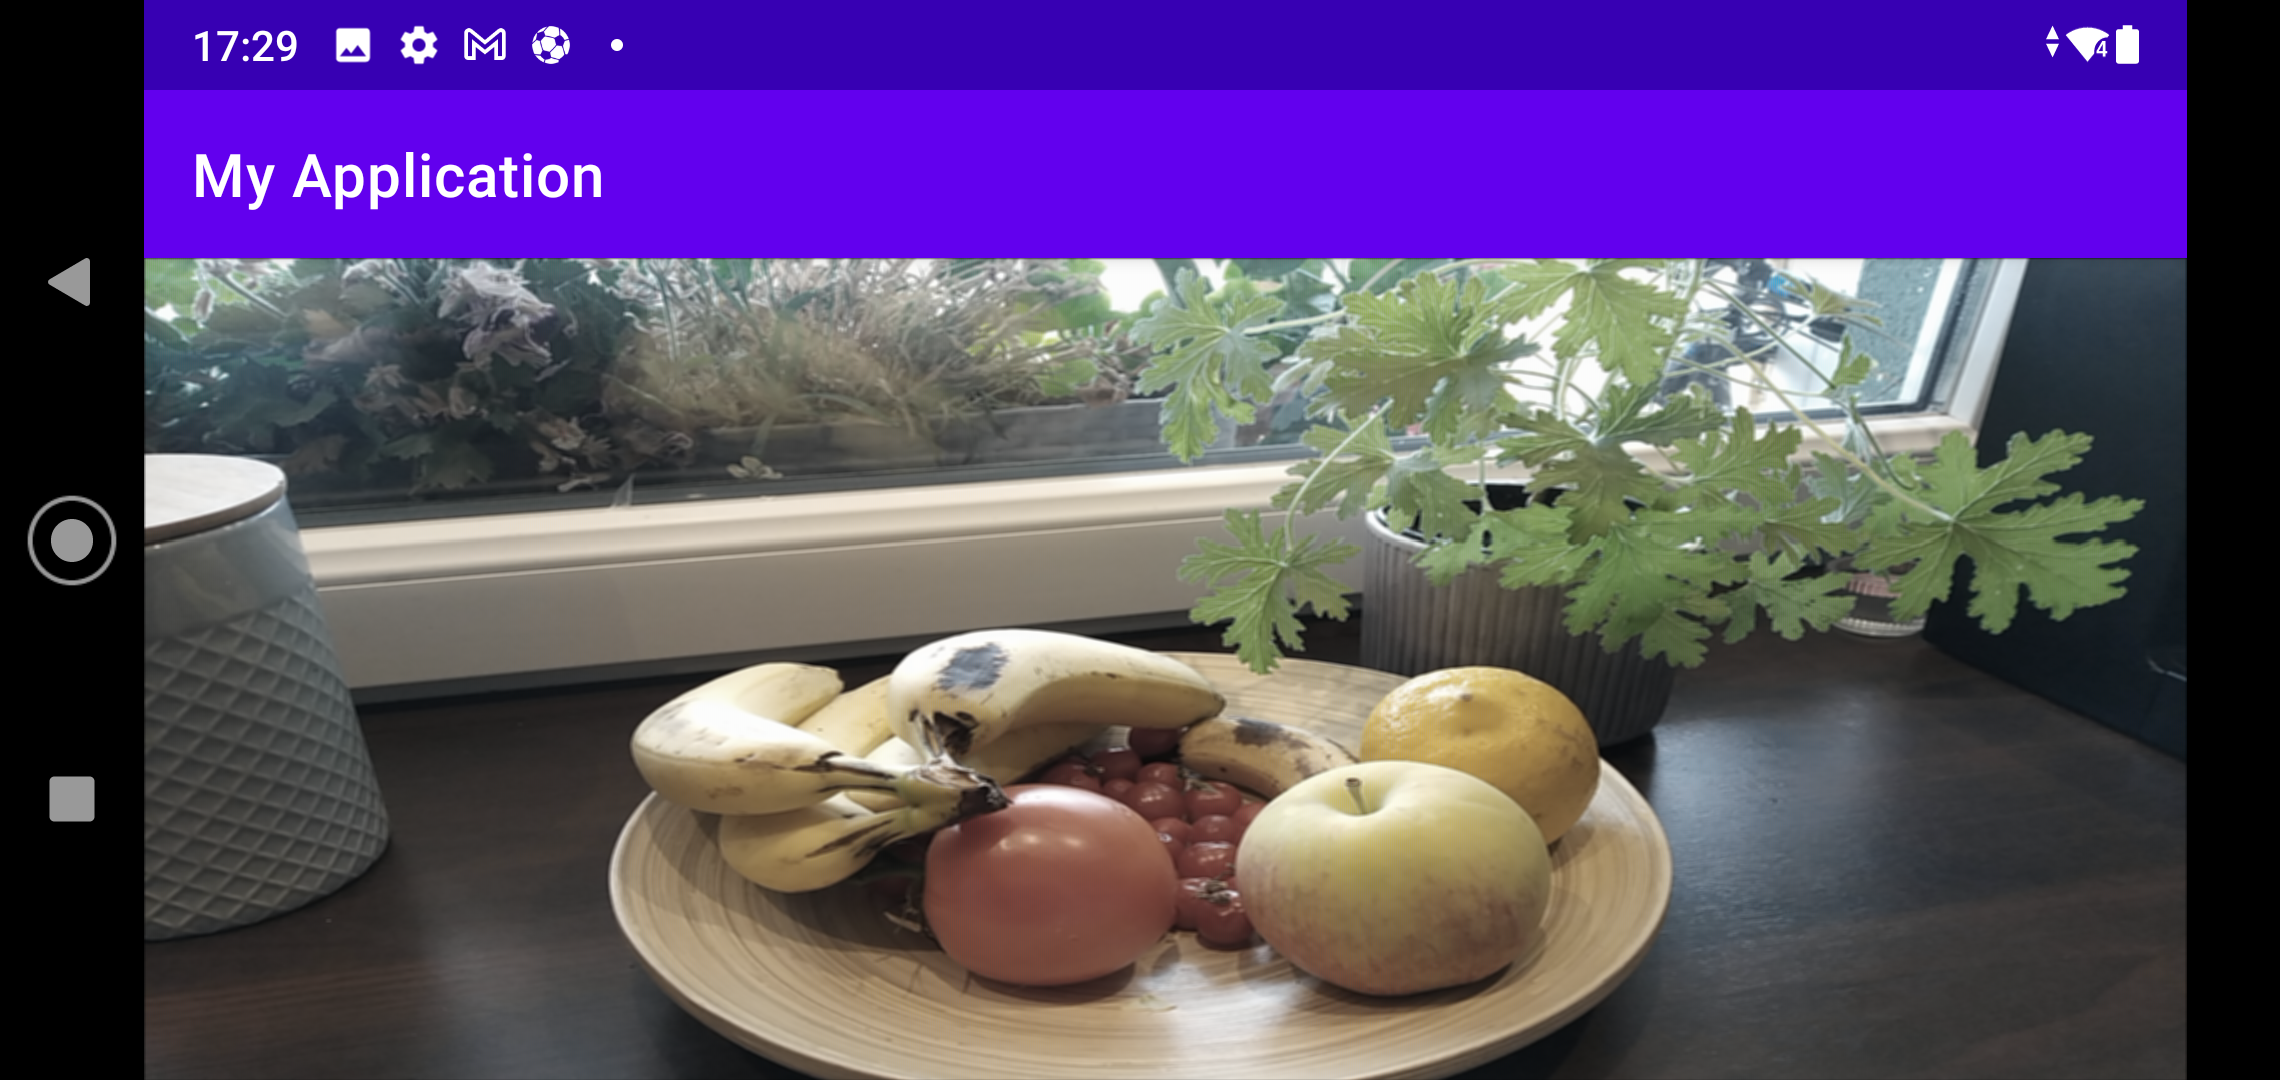
\includegraphics[scale=0.16]{imgs/avgFilter.png}
	\caption{Podgląd z filtrem uśredniającym}
\end{figure}
